\chapter{Testovanie a výsledky}

\section{Kritériá a popis testovania}
\subsection{Vstupné dáta}
Častým problémom pri vzájomnom porovnávaní algoritmov je
nájsť testovaciu vzorku, ktorá by otestovala beh algoritmu na širokej škále grafov.
Ako bolo v úvode spomenuté, súťaž {\sl Grid-Based Path Planning Competition} poskytuje množstvo máp rôznych typov a rozmerov,
na ktorých sa algoritmy dajú testovať. Formát máp popisuje napr. \cite{sturtevant2012benchmarks}.

Programy boli testované na dvoch mapách. Ich grafická reprezentácia bola 
vytvorená pomocou programu T-map(popis programu sa nachádza v prílohe \ref{userdoc}) 
a~môžme ju vidieť na obrázkoch Obr.~\ref{fig:aftershock_map} a~Obr.~\ref{fig:brushfire_map}.

\begin{figure}[h]
\centering
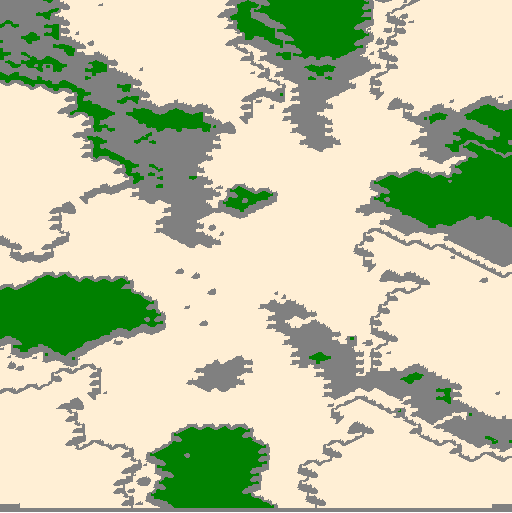
\includegraphics[width=10cm]{./img/Aftershock.png}
\caption{Graf \uv{Aftershock}}
\label{fig:aftershock_map}
\end{figure}
\begin{figure}[h]
\centering
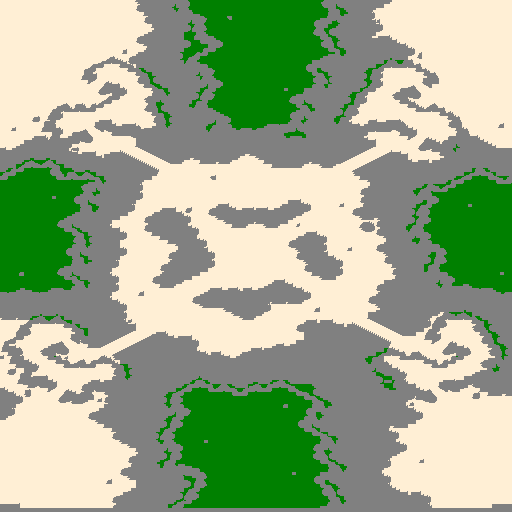
\includegraphics[width=10cm]{./img/Brushfire.png}
\caption{Graf \uv{Brushfire}}
\label{fig:brushfire_map}
\end{figure}
\subsection{Testovacie kritériá}
Testovacie kritéria sú podobné ako testovacie kritériá v súťaži. 
Odlišujú sa z dvoch dôvodov. TODO?? prvych 20 krokov je nezmysel + pridal som niektore veci navyse

\begin{itemize}
\item Počet prehľadaných vrcholov.
\item Rýchlosť nájdenia cesty.
\end{itemize}


\subsection{Testované algoritmy}
Testovať budeme nasledujúce algoritmy:
\begin{itemize}
\item Dijkstrov algoritmus nad binárnou haldou.
\item Dijkstrov algoritmus nad priehradkovou haldou.
\item A* používajúc rôzny počet landmarkov.
\item A* používajú optimálny počet landmarkov a obdĺžnikovú dekompozíciu.
\item TODO?? nieco dalsie blablabla - cudzie algoritmy zo sutaze
\end{itemize}


\subsection{Kompilácia}
Kód bude kompilovaný kompilátorom g++. Bude porovnaná
rýchlosť behu programu pri kompilácii s direktívami \emph{g++ -march=native -O3}, čo zaručuje maximálnu rýchlosť a efektivitu behu kódu.

\subsection{Typy máp a ciest}
Algoritmy budú testovane na troch mapách. 
Ich grafická reprezentácia je vytvorená v programe T-maps.
Popis programu sa nachádza v prílohách ~\ref{userdoc}~\ref{programdoc}.







(ASK?? poet prehladanych vrcholov nie je kriterium, ktore dokazem testovat na cudzich algoritmoch - musel by smo do nich zahat a pridavat tam funkciu, ktora to pocita - co mam robit? mam pocet vrcholov testovat len na mojich algoritmoch?)




Na porovnávanie využijeme benchmark

TODO?? bibliografia styl - priezvisko,meno - alebo naopak???